%% Document setup for the manuscript.
%%
%% HAND-WRITTEN. emit_tex.py injects the title block between the markers
%% below and appends the body, but everything in this file is maintained by
%% hand -- typography is exactly the kind of thing that should be edited
%% where you can read it, not buried in a Python string literal.
%%
%% Compile with:  xelatex main.tex   (twice, so figure references settle)

\documentclass[11pt,a4paper]{article}

\usepackage[margin=2.8cm]{geometry}

%% XeLaTeX with unicode-math, not pdflatex. The prose already carries Greek
%% letters and relations as Unicode, and unicode-math typesets them properly
%% instead of forcing a transliteration table at the emitter.
%%
%% amssymb is deliberately absent. unicode-math defines \eth, \digamma,
%% \backepsilon and \smallsetminus itself, and loading both makes LaTeX abort
%% with "Command already defined".
\usepackage{fontspec}
\usepackage{unicode-math}
\setmainfont{Latin Modern Roman}
\setmathfont{Latin Modern Math}

\usepackage{amsmath,amsthm}
\usepackage{graphicx}
\usepackage{caption}
\usepackage{fancyhdr}
\usepackage[htt]{hyphenat}
\usepackage[hidelinks]{hyperref}

%% Paragraph rhythm. A first-line indent with no inter-paragraph skip is the
%% convention in this field: it signals a new paragraph without inserting
%% white space the reader has to cross. The Word path set both as literal twip
%% counts in C#, which is what made the spacing read as loose and uneven.
\setlength{\parindent}{1.2em}
\setlength{\parskip}{0pt}
\linespread{1.08}

%% Lean declaration names run long -- scale_by_new_layers_not_by_headcount is
%% wider than the text block -- and a typewriter word has no break points by
%% default, so one would overhang the margin by 160pt. [htt] in hyphenat
%% above lets \texttt hyphenate, and the extra stretch lets TeX loosen
%% interword space rather than push a word into the margin.
\emergencystretch=3em

%% The paper's claims are stated as definitions and theorems, so they get
%% numbering and can be referred to by name rather than by "the paragraph
%% after equation 2".
\theoremstyle{definition}
\newtheorem{definition}{Definition}
\newtheorem{theorem}{Theorem}
\theoremstyle{remark}
\newtheorem{remark}[definition]{Remark}

\captionsetup{font=small,labelfont=bf,skip=6pt}
\captionsetup[figure]{labelsep=period}

%% Running head.
\pagestyle{fancy}
\fancyhf{}
\renewcommand{\headrulewidth}{0.4pt}

\begin{document}

%% The markers sit after \begin{document} on purpose. \title and \maketitle
%% are only legal once the document body has started; putting them in the
%% preamble makes LaTeX stop with "Missing \begin{document}".

%% BEGIN TITLE BLOCK -- replaced by emit_tex.py
\fancyhead[L]{\small Two saturating operators}
\fancyhead[R]{\small\thepage}

\title{\textbf{Two saturating operators: non-substitutability of human and machine contribution in AI-assisted discovery}}
\author{Huan Li\\ \small Independent Researcher\\[6pt]        \small ORCID 0009-0004-2695-6825\\ \small doi:10.5281/zenodo.23276356}
\date{}

\maketitle
\thispagestyle{fancy}
%% END TITLE BLOCK
\begin{abstract}
Humans and AI systems are usually placed on one capability curve and asked who is ahead. That framing has no formal content and it produces the wrong advice. The two parties act on different variables, and each saturates on a different axis.
We formalize the alternative. A machine, holding the hypothesis space fixed, compresses the residual toward a floor it cannot pass: the total gain is bounded by $log(e_0/Φ)$ and does not improve with more inference steps. A human, holding the hypothesis space fixed, moves the floor itself, and the gain from doing so is unbounded. Two further saturations fall out of the same currency. Headcount saturates immediately: under a max-type coalition the N+1th member's gain is exactly zero while its cost is exactly $log(Φ/a)$. And corpus size saturates too, because only the single item certifying the lowest floor determines the attainable bound, and a corpus whose published items are all bounded below by c can never certify a floor below c, whatever its length.
Three layers of content-level and system-level mathematics sit underneath, and they are what make the claim checkable rather than rhetorical. Total variation is the exact maximal discriminability available to any detector, so verification effort has a floor that no amount of reviewer diligence lowers. Truth is an equivalence class induced by the observation protocol, which splits human and machine contribution into two currencies with no monotone exchange rate between them. And the sign of the leading information-theoretic measure of human contribution is not identified: the same output is reported as $−0.099$ under one calibration and +0.169 under another.
All 153 theorems and 20 worked examples are machine-checked in Lean 4 (v4.15.0) against Mathlib, with zero sorry and zero admitted axioms beyond Classical.choice, Quot.sound and propext.
\end{abstract}
\section*{1  The claim}
The useful question about AI in science is not whether the machine has become good at the work. It is which part of the work it is good at, and what that leaves unclaimed. Answering that requires separating two operations that are routinely run together and priced in the same currency.
A machine that has been shown a mechanism hypothesis compresses the distance between the current estimate and the best estimate the protocol can certify. That is a bounded operation: the floor is set by the protocol, and no amount of sampling, ensembling or calibration crosses it. A human who notices that the mechanism should be measured at a different resolution changes which estimates are attainable at all. That operation moves the floor, and there is no ceiling on how far it can be moved.
The two are not two points on a shared scale. They act on different variables, which is why the standard question, how much of the work can be handed over, has no answer that stays stable under refinement. More of the machine's operation cannot move the quantity the human's operation acts on. The bottleneck relocates from speed to layer selection and verification, and it does not stay there.
Three consequences follow, and each is a theorem rather than a position. Within a fixed hypothesis space, the machine's total contribution has a hard ceiling that does not depend on how many steps were taken. Under a max-type coalition, additional people add cost and no reach. Under corpus growth, only floor-lowering material counts. Each has a stated falsification condition, given in section 8.
\section*{2  Two operators, two saturation axes}
Work through the layer machinery first, since the later sections borrow its currency. Fix an observation protocol at resolution $α$. It induces an equivalence relation on states, and the true state is the class of states the protocol cannot resolve. Within a layer, the attainable estimates form a reachable set R, and the certified coverage of the true state within its class is the floor $Φ$, the infimum of distance over that reachable set.
The reachable set must be restricted for this to be non-degenerate. Without that restriction one may take an estimate inside the true state's own class, obtain $Φ$ = 0, and every logarithmic decomposition below collapses to a triviality. We state this as a modelling commitment rather than a theorem, and return to it in section 8.
Error then decomposes into a ceiling term and a within-layer term, and the two summands are not commensurable.
\begin{equation}
\underbrace{\log\!\frac{\Phi(\alpha)}{\Phi(\beta)}}_{\text{\rm refinement: moves }\Phi\ \text{--- unbounded above}}\qquad\qquad\underbrace{\sum_{t}\log\!\frac{e_{t-1}}{e_t}}_{\text{\rm compression: moves } e_t\ \text{to }\Phi}\ \leq\ \log\frac{e_0}{\Phi}
\tag{1}
\end{equation}
Refinement contribution is human work that moves the certified coverage itself, changing the target. Its gain is unbounded above: for any target M $≥$ 0 there are two layers with $Φ(β)$ $≤$ $Φ(α)$ and $log(Φ(α)/Φ(β))$ = M \texttt{(human\_gain\_unbounded)}.
Within-layer compression is machine work that moves the residual to that target, changing the distance to it. Its total is bounded, and the bound contains no variable appearing on the other side.
\begin{equation}
\log\!\frac{e_0}{e_N}\ \leq\ \log\!\frac{e_0}{\Phi}\qquad\text{fixed by the layer, independent of the number of steps}
\tag{2}
\end{equation}
This is stronger than the observation that per-step marginal gain vanishes. The per-step sum converges to a finite limit that the layer itself fixes.
\begin{equation}
\text{within-layer gain}\;\leq\;\log\!\frac{e_0}{\Phi}\qquad\text{while}\qquad\text{refinement gain}\;>\;K\quad\text{for every }K\geq 0
\tag{3}
\end{equation}
\texttt{saturation\_duality} places the two side by side and is the formal content of non-substitutability. Both sides saturate; the axes are different. No reweighting converts one into the other, because the bound on one side contains no variable appearing in the other. Separately, the convexity of scaling-law cost makes partial automation a long-run cost-minimizing equilibrium rather than a transitional state [17], which is an economic reason to expect the split to persist rather than close.
\begin{figure}[tb]
\centering
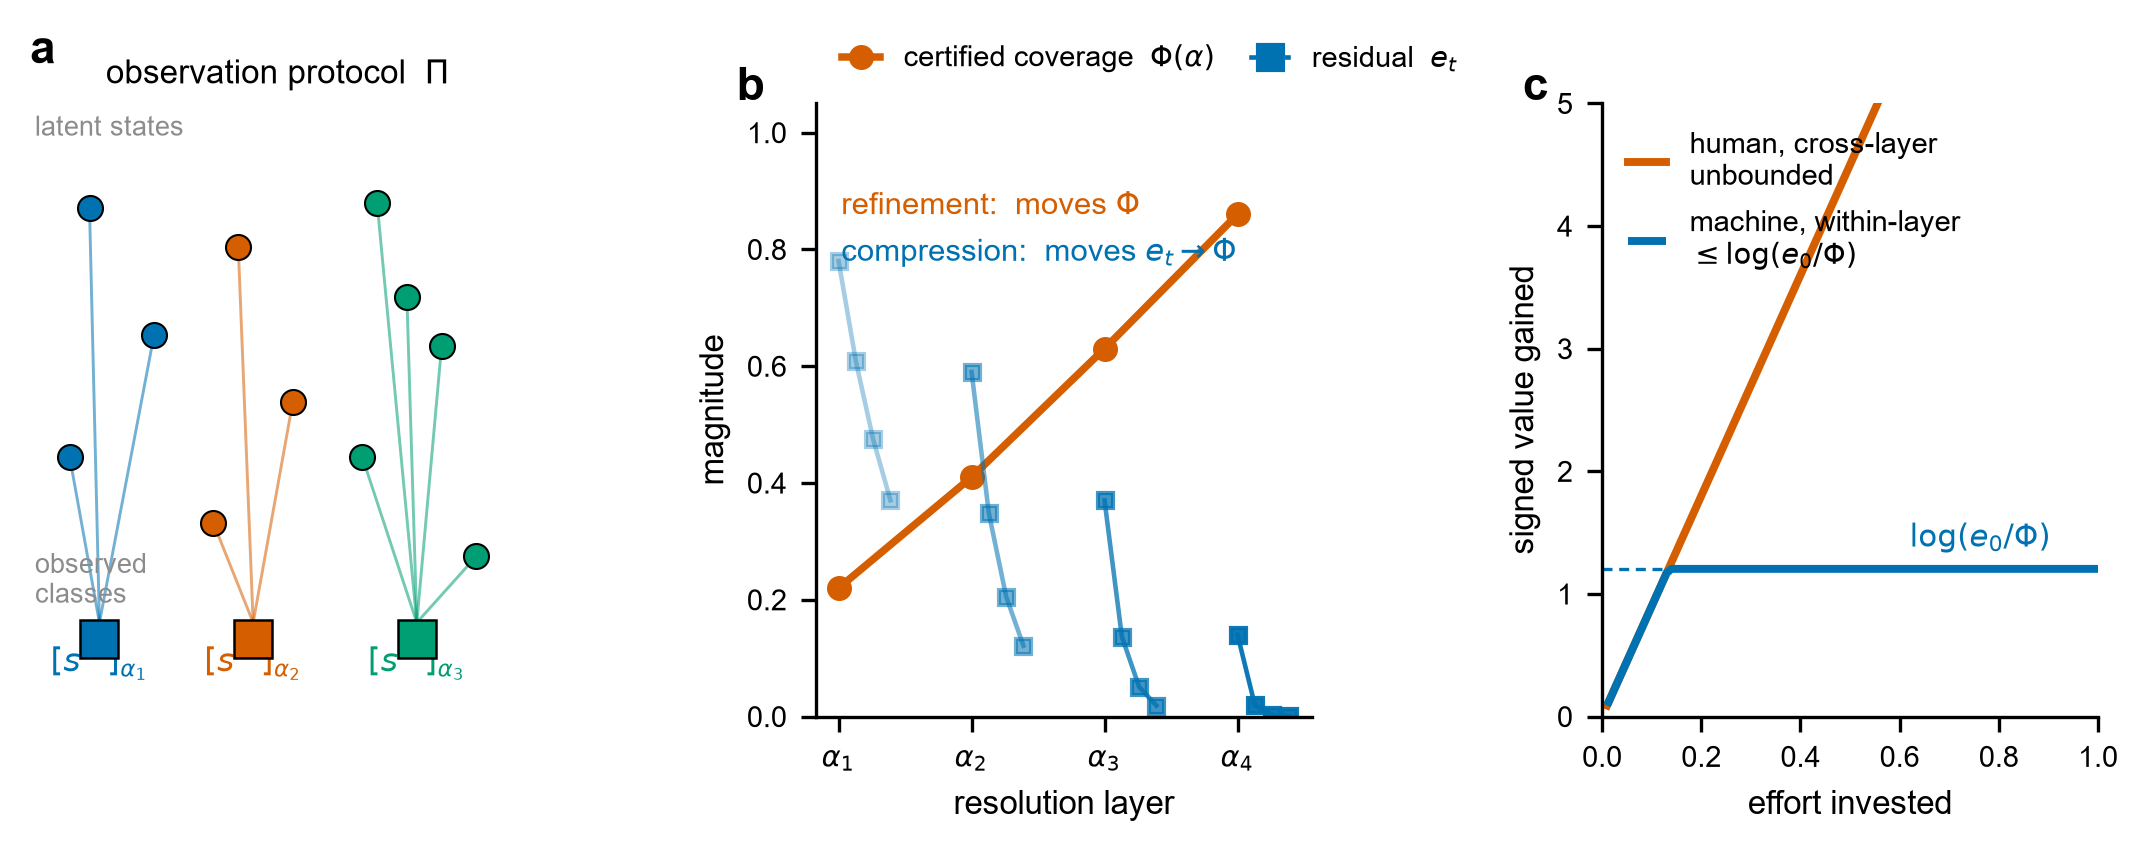
\includegraphics[width=6.10in]{../figures/fig3_layers.png}
\caption{The two operators. (a) The observation protocol induces an equivalence class [s*]; certified coverage $Φ(α)$ is a property of the class, not of a point. (b) Refinement (human, cross-layer) moves $Φ$ itself and has unbounded gain; within-layer compression (machine) reduces the residual $e_t$ to $Φ$ and is capped at $log(e_0/Φ)$. (c) The two curves have different shapes, which is what makes them non-convertible.}
\label{fig:layers}
\end{figure}
\section*{3  The content layer}
\subsection*{3.1  The best possible detector is already characterized}
Section 2 assumed a floor. This section derives it, for the case where the two competing hypotheses are concrete distributions. Let p and q be two distributions on a finite outcome space, and TV their total variation distance. Any procedure returning a binary call from a sample of p or q is a statistical test.
\begin{equation}
\mathrm{TV}(p,q)\;=\;\frac{1}{2}\sum_x \left|p_x-q_x\right|
\tag{4}
\end{equation}
\begin{equation}
\text{maximal excess accuracy}\;=\;\frac{\mathrm{TV}(p,q)}{2}\qquad \text{minimal error}\;=\;\frac{1-\mathrm{TV}(p,q)}{2}
\tag{5}
\end{equation}
Neyman-Pearson theory already answers how far such a test can go [5,6], and both bounds are attained rather than merely approached. This is Le Cam's two-point lemma, and it is the floor $Φ$ in the general case.
Two corollaries matter in practice. Reweighting, post-processing, ensembling and threshold tuning are already contained in the optimum, because the ROC geometry is fixed by p and q alone [7]. And the two-sided form |TP - FP| $≤$ TV is the identity J $≤$ TV for Youden's index J = Se + Sp - 1, not a modelling assumption [8,9].
One common error deserves a note, because it has the form of a theorem and is false. The inequality mass(p,S) + mass(q,S) $≥$ 1 + TV fails at S the whole space when p = q, where it reads 2 $≥$ 1. The correct identity is TP + FN = 1.
The consequence for AI-assisted biology is severe. As a generator's output distribution converges to the reference distribution, TV goes to zero and every attainable advantage goes with it. This is conditional on a convergence assumption that Silva et al. state explicitly and, to their credit, decline to claim has already occurred [10]; conditional on it, no architecture and no quantity of calibration data changes the conclusion. Their impossibility is not a new obstruction: it follows from classical results in statistical decision theory, and the contribution of their argument is to show that the generator-cooperation requirement, not the classifier, is what makes the obstruction bite [10].
The empirical literature has paid this bill twice. Recursive paraphrase attacks drove a strong watermarked-model detector from 99.8\% true-positive rate at a 1\% false-positive operating point down to 9.7\%, and a statistical detector from 96.5\% AUROC to 25.2\%, that is, to chance [11]. A single adversary suffices to defeat any watermark of a given detectability [12]. These are not failures of effort. They are the bound becoming visible.
\begin{figure}[tb]
\centering
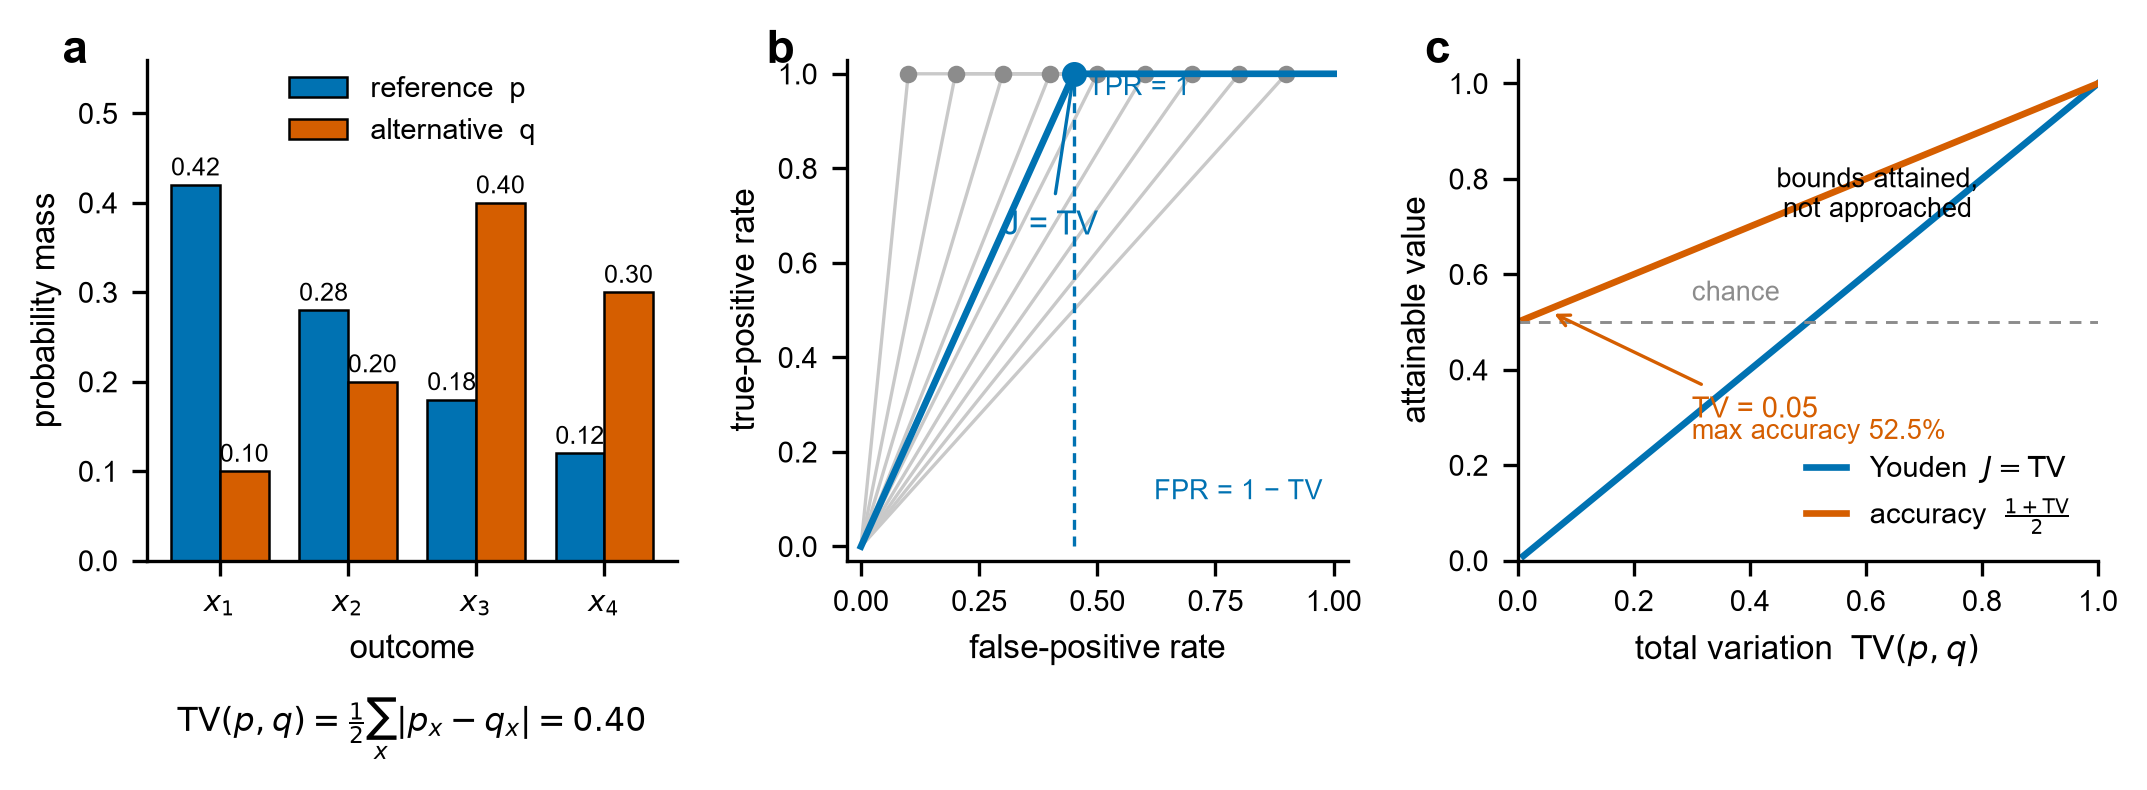
\includegraphics[width=6.10in]{../figures/fig1_ceiling.png}
\caption{The identifiability ceiling. (a) Every test of two hypotheses p and q is bounded by Le Cam's two-point lemma: the excess accuracy over chance is exactly TV(p,q)/2 and the error rate is exactly (1 - TV)/2. Both bounds are attained, so no detector can exceed the curve. (b) The two-sided form |TP - FP| $≤$ TV is the identity J $≤$ TV for Youden's index J = Se + Sp - 1; the geometry is fixed by p and q alone, leaving threshold choice no freedom. (c) As a generator's distribution converges to the reference distribution, TV $→$ 0 and attainable advantage $→$ 0, independently of detector architecture.}
\label{fig:ceiling}
\end{figure}
\subsection*{3.2  Verification effort has a floor}
The natural next move is to ask whether verification escapes the bound. Repeatedly checking a candidate should accumulate evidence the way repeated surveys accumulate detection probability. It accumulates, up to a floor.
Suppose a reviewer of reliability p inspects a candidate, a machine checks it with per-round detection probability q, and N rounds cost c each. The naive residual miss rate (1 - $q)^N$ decays geometrically to zero, which cannot be right: a genuinely zero residual would give the verifier perfect discriminability and hence TV = 0. The corrected model adds an irreducible floor.
\begin{equation}
\text{miss rate}(N)\;=\;\max\!\left[\,(1-q)^{N},\;\lambda\cdot\mathrm{TV}\,\right]
\tag{6}
\end{equation}
Minimizing total cost R(N) = p*c + A*max[(1 - $q)^N$, T] + c*N with A = (1 - p)L, L the loss scale and T = $λ*TV$, gives an interior optimum N* = $min(N_c$, $N_0)$ bounded by
\begin{equation}
N^{*}\;\leq\;N_0\;=\;\frac{\ln\!\big(1/(\lambda\cdot\mathrm{TV})\big)}{\ln\!\big(1/(1-q)\big)}
\tag{7}
\end{equation}
a bound that contains no p whatsoever. Raising TV does not make review safer; it makes review cheaper, because distributions further apart saturate the verifier sooner and therefore need fewer rounds.
Dorner and colleagues prove related results in a different register, and the convergence is not ours. They show that the per-instance accuracy of verifier-driven test-time scaling is characterized by the geometry of the verifier's ROC curve, that rejection sampling and best-of-N share one large-compute limit set by the ROC slope at the origin, and that high-compute performance cannot be predicted from low-compute observations [13, Propositions 2, 3 and 7, Theorem 1]. Three differences remain. They characterize accuracy at a given compute C and never optimize over the budget, so no finite optimal round count appears in their analysis; in the regime that matters their compute cost C(F) diverges as F approaches zero. Their free parameters are the generator's initial accuracy pi and the ROC curve, with no parameter anywhere for the reliability of a human reviewer. And their plateau depends jointly on pi and the ROC slope at the origin, whereas T = $λ*TV$ is the separability of the two hypotheses and is independent of who performs the verification.
\begin{figure}[tb]
\centering
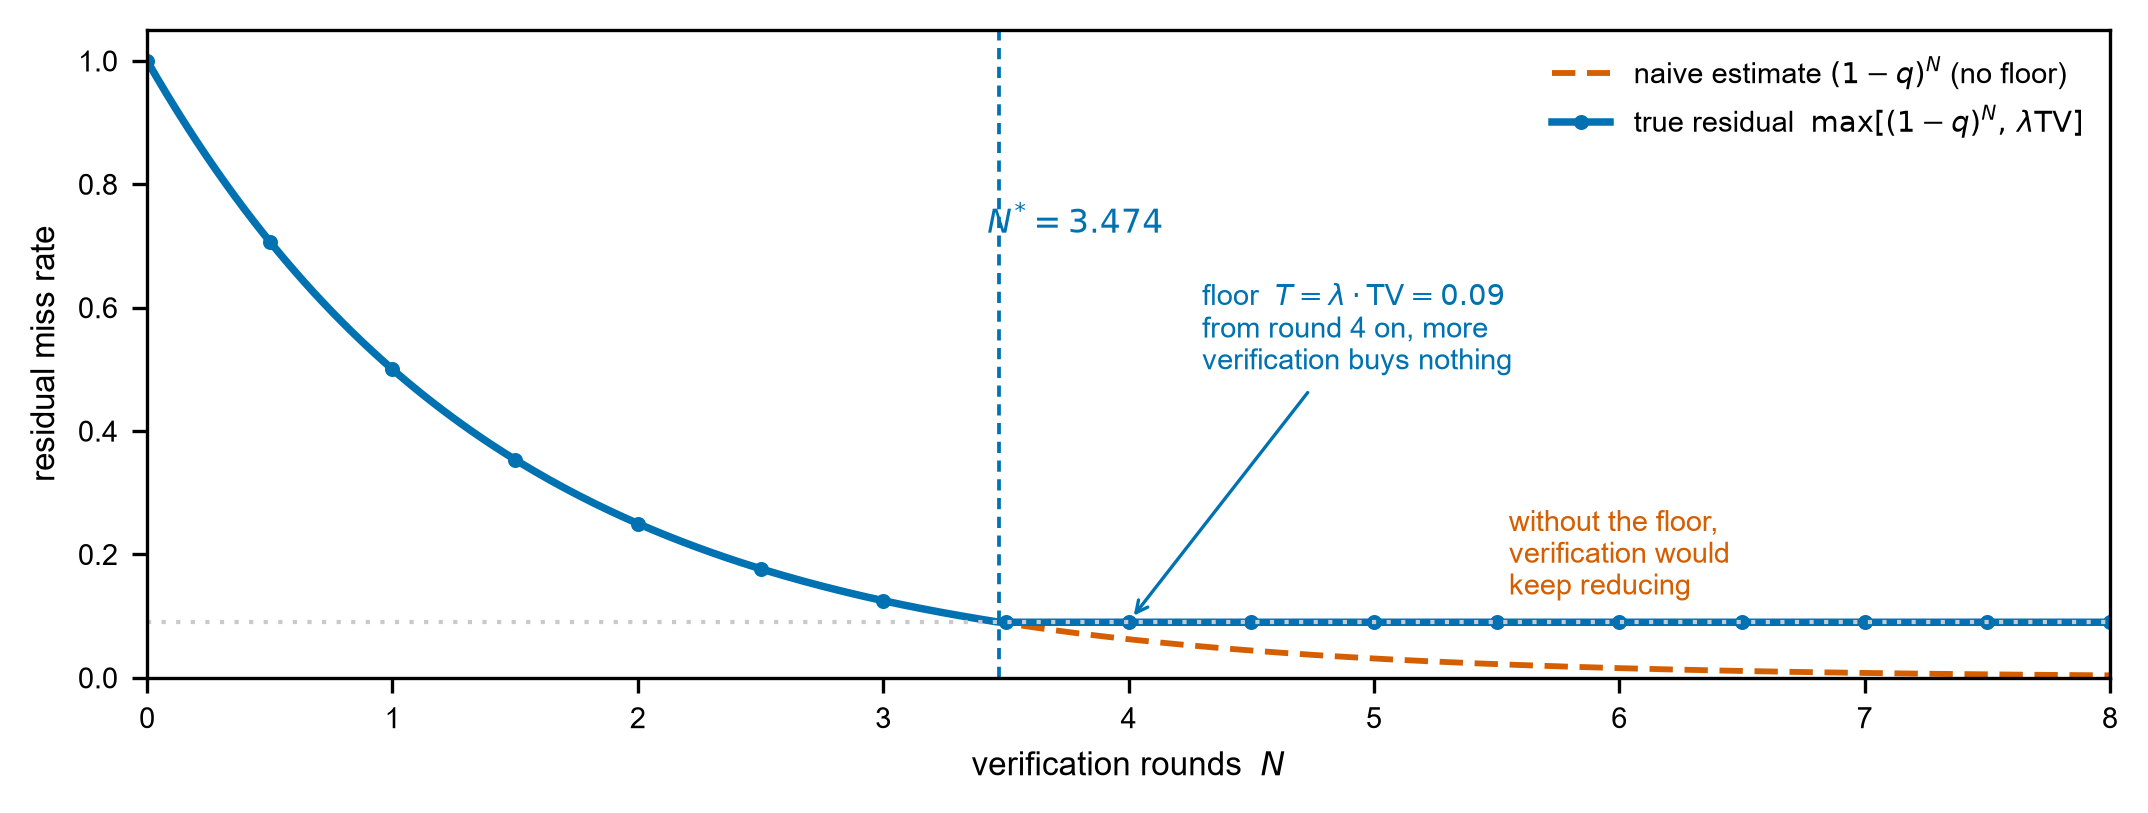
\includegraphics[width=6.10in]{../figures/fig5_verification_floor.png}
\caption{Verification effort has a floor. Residual miss rate decays geometrically as (1 - $q)^N$ and is then clipped at the floor T = $λ*TV$, giving the maximum of the two. The cost-minimizing budget N* is the smaller of the unconstrained optimum $N_c$ = 3.793 and the p-independent cap $N_0$ = 3.474, which binds here. Over the scanned parameter grid the floor is the active constraint in 83.97\% of combinations, where the bottleneck is the detector rather than the reviewer. Parameters: TV = 0.09, q = 0.5, $λ$ = 1.}
\label{fig:floor}
\end{figure}
\subsection*{3.3  An instantiation}
Cryptic sister species give the cleanest field demonstration. Two species may be separable by one fixed nucleotide, by one courtship call, or by nothing a given survey protocol can register. The first case is a fact about the organisms, the last a fact about the protocol, and the literature is careful to say which. Where two species differ only in features the protocol cannot register, they are not the same species; they are operationally equivalent for that survey. The same structure recurs across modern biology. Environmental DNA surveys trade sequence-discriminating power against a contamination-driven false-positive rate and a detection-driven false-negative rate. Homology modelling can leave a backbone well constrained while a functionally critical loop is not, and a confidence metric does not make the unconstrained region less so.
\section*{4  The system layer}
\subsection*{4.1  Truth is an equivalence class}
Under an observation protocol with an induced equivalence relation, the true state is the class, not a point. This is standard in representation learning, where observability is characterized by a quotient of the state space by a kernel [14,15] and by observation-induced equivalence in statistical experiments [16], and in survey design, where occupancy is a latent state and detection the observation model [1]. We take no novelty claim for the quotient itself. The consequence is unglamorous: a resolution limit is not fixed by acquiring more of the same observable, only by changing the observable.
\subsection*{4.2  The sign of a credit measure is not identified}
The sharpest formal statement concerns the measures now proposed for human contribution. The leading operational proposal is information-theoretic: human contribution is the proportion $φ$ = I(x;y)/I(y) of the self-information of the output shared with the human input, with I(x;y) = I(y) - I(y|x) and I(y) = -log p(y) [18, Definition 1]. The measure is carefully validated. It tracks engineered levels of human input across four domains and six models, and agrees with pairwise human annotation on 95.9\% of 1,500 pairs.
It is also, by construction, entirely unsigned. Every quantity entering it is a surprisal, both non-negative, and their difference is the only quantity used. There is no notion of direction in the definition and no hypothesis class in which the ratio would be well-posed.
We should be exact about what follows, because it is less dramatic than it first appears. The authors do not claim otherwise. Their limitations section states that the framework measures informational contribution, that informational contribution should not be directly equated with creativity or originality, that it is not a normative judgment about creative value or authorship, and that human editing may carry creative input it does not capture [18]. Their results are reported over settings in which measured human contribution ranges down to minimal or negligible human contribution [18, section 5.5]. The measure is not wrong for its stated purpose. What the separability result adds is a theorem where they supply a sentence: the caveat is an axiom-level property of the whole class, so the measure cannot be extended into credit accounting or originality adjudication by recalibration. Only a signed definition does that.
Rewriting their estimator exposes a sharper problem than the negatives. Their Equation (10) reduces to
\begin{equation}
\hat{\varphi}\;=\;\frac{I(y)+N\log\tau}{I(y)}\;=\;1-\frac{\bar{\tau}}{\bar{s}},\qquad \bar{\tau}=-\log\tau,\quad \bar{s}=\frac{I(y)}{N},\qquad \hat{\varphi}<0\iff\bar{s}<\bar{\tau}
\tag{8}
\end{equation}
Two consequences follow. The estimator is a function of the output alone, since the human input does not appear, and it is unbounded below as the output grows more predictable, so the [0,1] reading does not survive in the estimation variant. And its sign is determined by whether the mean per-token surprisal falls below the plausibility bar, where that bar is fitted rather than measured: the authors set it to the empirical mean plus one standard deviation of conditional surprisal over 2,500 WildChat prompts, giving 0.5496 for Llama-3 and 0.4155 for Mixtral [18, section A.5].
The only sign this framework can report is therefore set by a nuisance parameter estimated out of distribution. The same output is evidence of contribution under one calibration and evidence against it under another. \texttt{sign\_not\_identified} exhibits two calibrations that flip the reported sign for any output; \texttt{sign\_not\_identified\_exact} pins the witnesses to bars at half and one-and-a-half times the output's mean surprisal. The apparent sign is a property of the calibration, not of the collaboration.
\begin{figure}[tb]
\centering
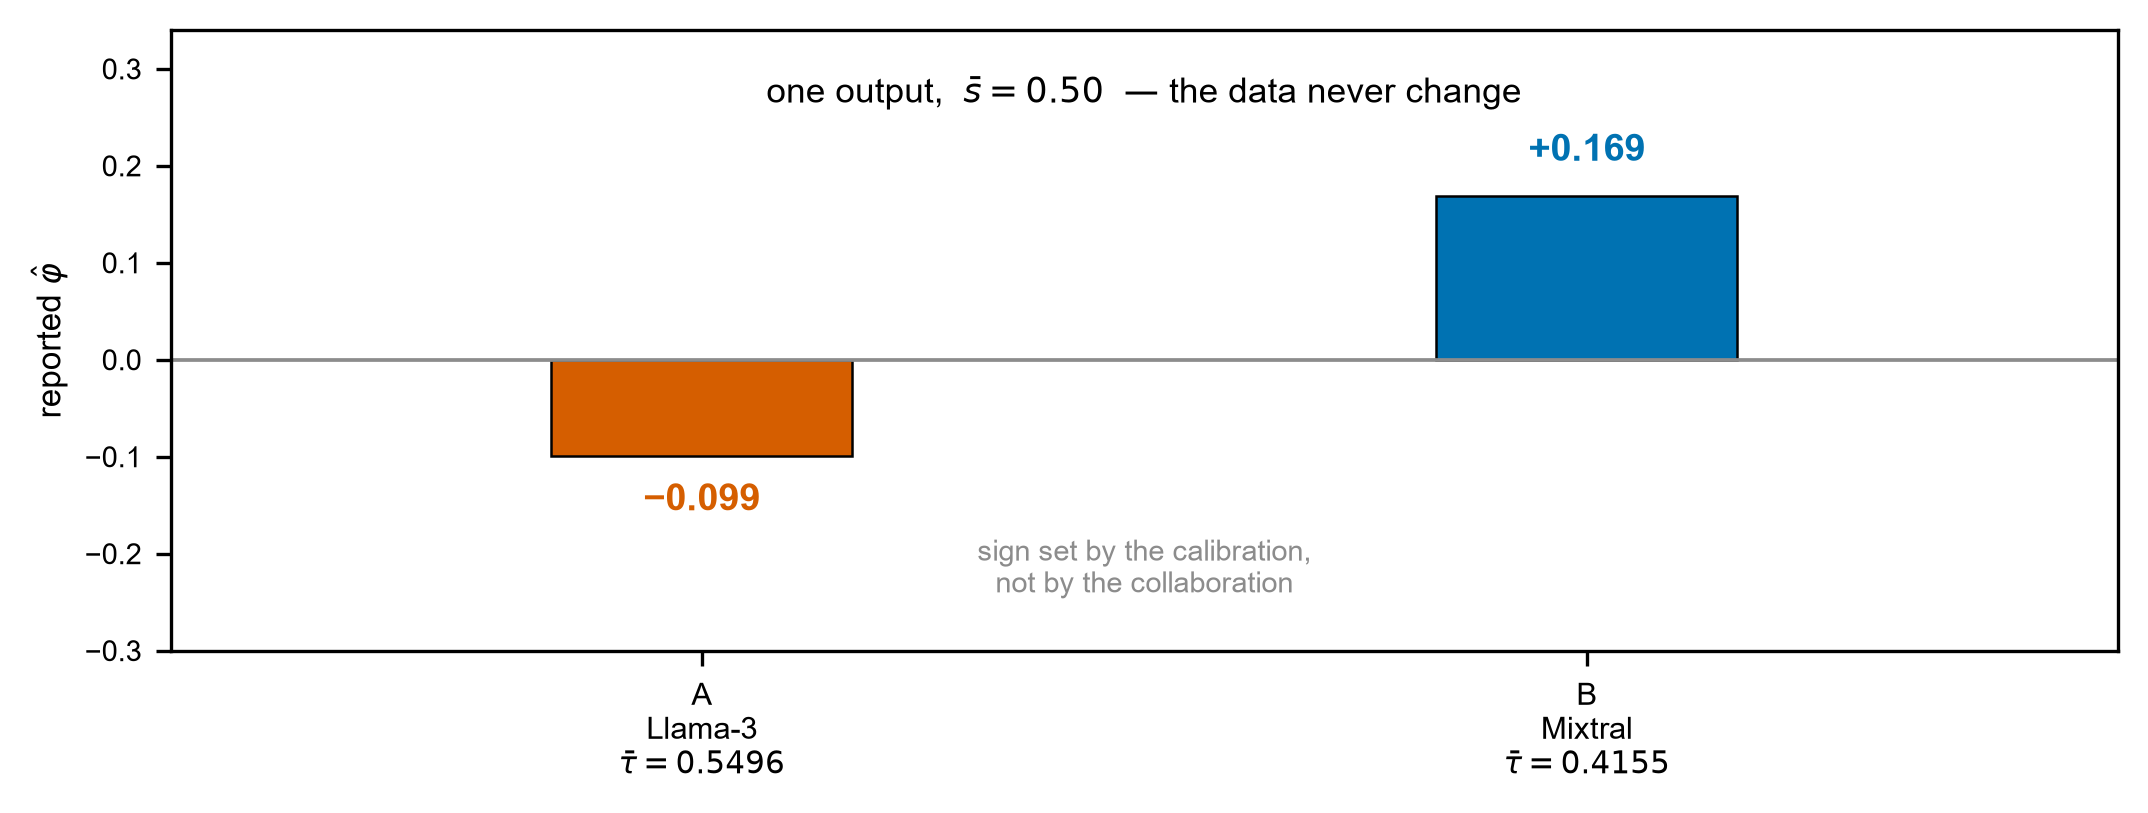
\includegraphics[width=6.10in]{../figures/fig6_sign_not_identified.png}
\caption{The sign of a credit measure is not identified. The estimated contribution $φ-hat$ = 1 - $τ-bar/\bar{s}$ is plotted as the plausibility bar $τ-bar$ moves through the plausible range. Because the estimator depends on the output alone and the bar is fitted out of distribution, the same output crosses zero: Llama-3 reports $−0.099$ at $τ-bar$ = 0.5496 and Mixtral reports +0.169 at $τ-bar$ = 0.4155. The witnesses that flip the sign are pinned at $τ$ = s/2 and $τ$ = 3s/2.}
\label{fig:sign}
\end{figure}
More generally, every reflection-invariant measure, KL, mutual information, total variation, Jensen-Shannon, has this blind spot as a property of the class rather than of an implementation. An author who moves a claim toward the truth and one who moves it toward an equally plausible falsehood produce identical mutual information with the text.
\begin{equation}
\left|\mathrm{influence}\right|\;=\;m\quad\Longrightarrow\quad\mathrm{value}\;=\;+M\ \ \text{or}\ \ -M,\qquad \forall M>0
\tag{9}
\end{equation}
\texttt{influence\_value\_separable} makes this exact: for any M > 0 there are processes with identical absolute influence between two states whose signed value is +M, and processes with the same absolute influence whose value is -M. The measure returns the same number; the biology has moved in opposite directions.
This also refutes the natural first attempt at a within-layer sensitivity function, the absolute change in $Φ$ with respect to x. Taking an absolute value identifies refinement with coarsening, so the instrument cannot distinguish an author who sharpened a mechanism model from one who blurred it, and reports zero for both.
The fix is a signed definition fixed in advance, on order-preserving, additive, unit-fixing maps over a signed domain rather than arbitrary monotone transforms. Under that restriction the impossibility sharpens: when the floor binds, reviewers of different reliability produce identical optimal verification effort, and no monotone exchange rate between human bits and machine rounds survives. When it does not bind, the two are exponentially but not linearly related, exp(d*N*) = A*d/c. 'Fully incommensurable' overstates that second regime; 'not linearly convertible' is exact.
\begin{figure}[tb]
\centering
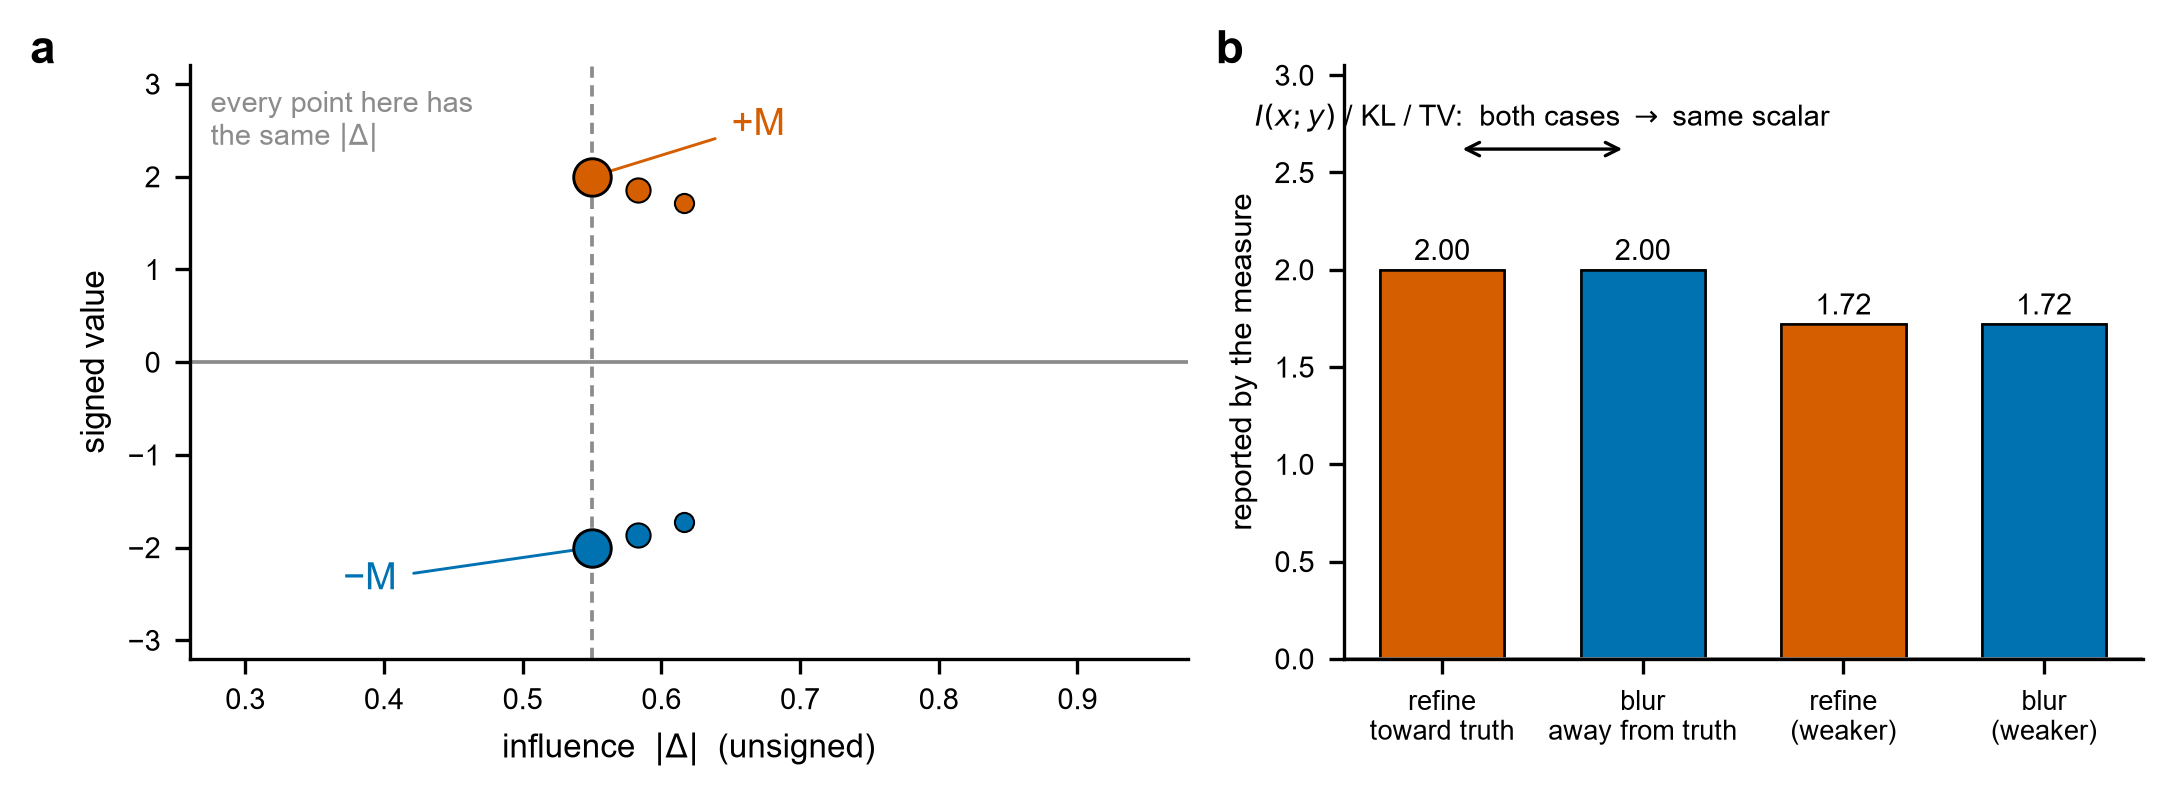
\includegraphics[width=6.10in]{../figures/fig4_separable.png}
\caption{Influence and value are separable. For any M > 0 there exist processes with identical |influence| between two states whose signed value is +M, and processes with the same |influence| whose value is -M. The horizontal coordinate (magnitude of change) is identical across all four cases; the vertical coordinate (signed contribution) is not determined by it. Any reflection-invariant measure - mutual information, KL, total variation, Jensen-Shannon - is blind to this split.}
\label{fig:separable}
\end{figure}
\section*{5  Saturation on the human axis: headcount}
Section 2 saturates the human operator in one direction, the floor across layers. It says nothing about the other direction, people. The obvious hope is that more researchers compress that axis, the way more inference steps compress the machine's. They do not.
Model a collaboration as the set of layers its members reach independently, with the joint result taken as the best of them. This is a max-type coalition, and it is a stronger claim than a discounted merge: it asserts that the merge is exactly the best individual and that every other member contributes exactly zero.
\begin{equation}
\mathrm{gain}(\Phi,D\cup\{a\})\;=\;\mathrm{gain}(\Phi,D),\qquad \mathrm{totalIndividual}(\Phi,D\cup\{a\})\;=\;\mathrm{totalIndividual}(\Phi,D)+\log\frac{\Phi}{a}
\tag{10}
\end{equation}
The N+1th person earns exactly zero and costs exactly $log(Φ/a)$. Define the waste as the difference between the summed member gain and the coalition gain. Then \texttt{waste\_nonneg} and \texttt{headcount\_adds\_waste\_only} say the merge never produces more than the best individual, and headcount only adds waste.
The time axis behaves the same way. Holding an increment back is not an option in the usual sense: the value of waiting is zero if the window is superseded by the time the delay arrives, and the full value otherwise. Coverage is absorbing, so once superseded, always superseded, and \texttt{holdValue\_antitone} says the value of waiting is non-increasing in the delay. There are two outcomes, not yet superseded and already superseded, and no third.
\texttt{fragmentation\_squeeze} closes both routes at once, and \texttt{scale\_by\_new\_layers\_not\_by\_headcount} names the remaining exit: scale by changing the layer, which is the unbounded direction of section 2.
The max assumption is the load-bearing part, and it is falsifiable in one move. If real collaboration is superadditive, if two people together reach a layer neither reaches alone as complementary expertise plausibly suggests, then \texttt{add\_member\_same\_reach} fails immediately. We state the assumption because leaving it to intuition invites exactly the recombination story the model denies.
\begin{figure}[tb]
\centering
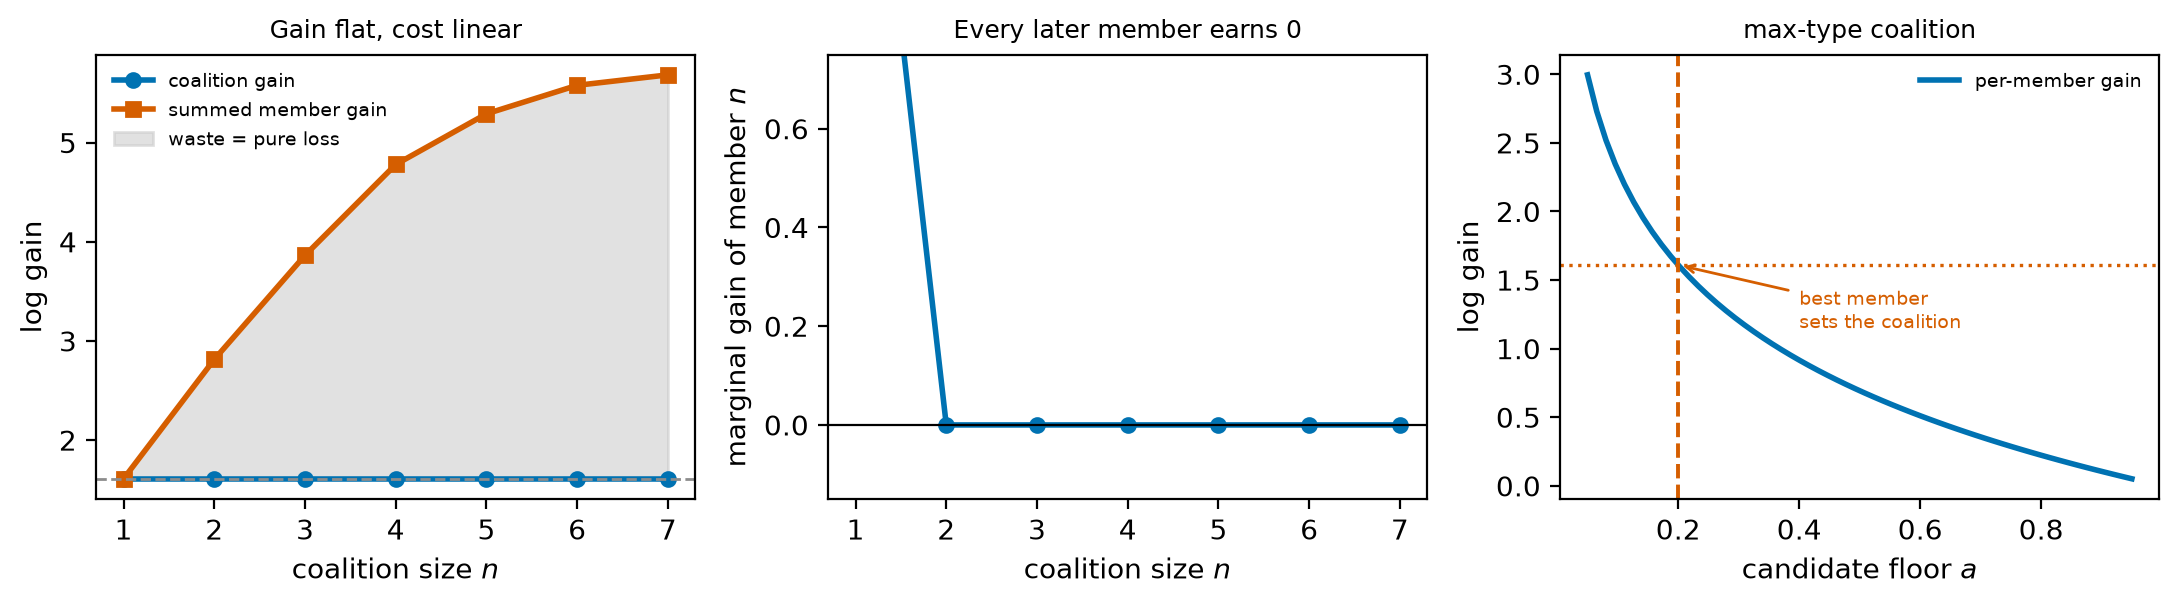
\includegraphics[width=6.10in]{../figures/fig5_headcount_saturates.png}
\caption{Headcount saturates immediately. (a) Coalition gain is flat in the number of members while the summed individual gain grows linearly; the band between them is pure waste. (b) The marginal gain of every member after the best one is exactly zero. (c) Under a max-type coalition the best member alone sets the outcome for every candidate floor.}
\label{fig:headcount}
\end{figure}
\section*{6  Saturation on the data axis: the corpus}
The same structure reappears on the data side, and it bears directly on a common claim about the AI era: that unread knowledge will in time become training material and therefore will not be lost. The quantity in doubt is not the size of the corpus, which grows without bound, but how much of it is usable.
Model a corpus as the set of floors its individual items certify, with the certified floor the best one on offer.
\begin{equation}
\mathrm{floorOf}(D)\;=\;\min D,\qquad\mathrm{floorOf}(D_1\cup D_2)\;=\;\min\big(\mathrm{floorOf}(D_1),\mathrm{floorOf}(D_2)\big)
\tag{11}
\end{equation}
Then the floor is determined entirely by the best item. \texttt{floorOf\_union\_le\_left} and \texttt{floorOf\_union\_le\_right} say that adding a corpus changes the joint floor only through that corpus's own best item, and \texttt{floorOf\_union\_self\_mono} covers arbitrary growth: add n items, none of which beats the existing floor, and the floor stays put. This is dilution invariance, and it says that a corpus which is ninety-nine parts filler and one part signal certifies precisely what the one part certifies. \texttt{uninformative\_corpus\_gains\_nothing} is \texttt{no\_gain\_without\_floor\_drop} at the corpus level: switching corpora without lowering the floor pays exactly zero.
The selection version is the sharper half. If every published item is bounded below by c, then the attainable gain is capped uniformly in the residual.
\begin{equation}
\big[\ \forall a\in D,\ c\leq a\ \big]\ \Longrightarrow\ \log\frac{e_0}{e_N}\;\leq\;\log\frac{e_0}{c}\qquad\text{uniformly in }e_N
\tag{12}
\end{equation}
\texttt{corpus\_size\_cannot\_beat\_selection\_floor} reads this contrapositively: no corpus, however large, certifies a floor below c if none of its items does. Corpus growth is unbounded; the floor it can certify is not. So the two halves of the usual claim come apart. Everything articulable does eventually enter the corpus. Whether it enters the usable part is settled by whether it lowers the floor, and that is a property of the item, not of its volume.
Two things are deliberately left out, and the omissions are the point. Whether a given artefact is articulable at all is not representable at this level, so the tacit-knowledge filter cannot be stated as a theorem. And the corpus is modelled as a set; nothing here says the best item is reachable, or that it is weighted up once found. Those are commitments, recorded in section 8.
\begin{figure}[tb]
\centering
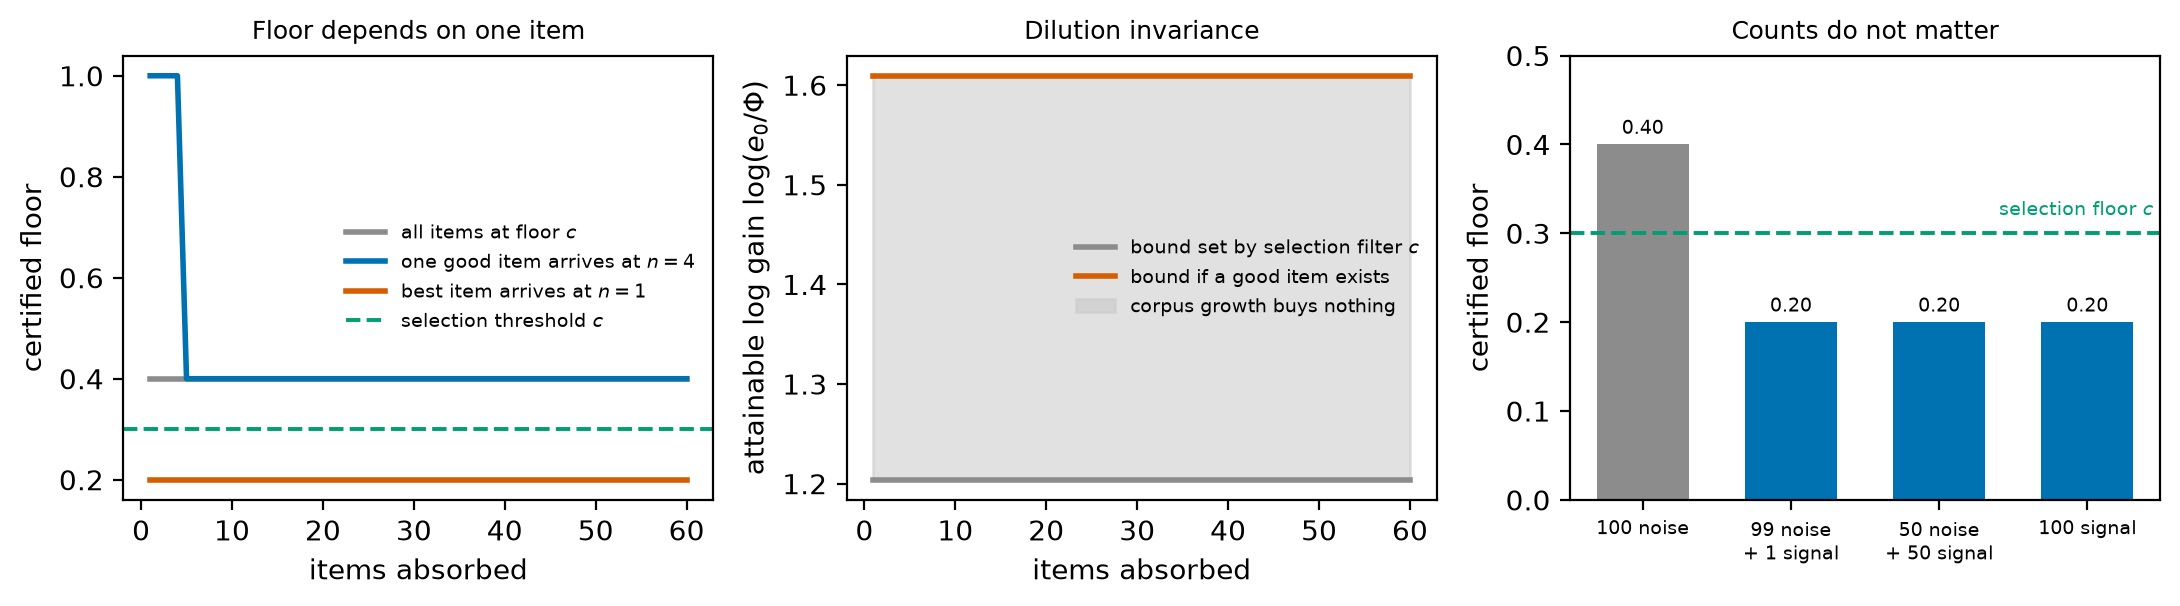
\includegraphics[width=6.10in]{../figures/fig6_corpus_saturates.png}
\caption{Corpus growth saturates too. (a) The certified floor depends on the single best item, not on how many items exist: a corpus in which the one good item arrives late reaches the same floor as one in which it arrives first. (b) The attainable log gain is pinned the moment one floor-lowering item exists; further absorption buys nothing. (c) For a fixed size of 100 items, the certified floor is 0.20 whether the corpus holds 1, 50 or 100 good items, and 0.40 when it holds none. The green line marks a selection floor c that no amount of growth can cross.}
\label{fig:corpus}
\end{figure}
\section*{7  What the 2026 evidence supports, and what it does not}
The formal claims make predictions, and the empirical literature of 2026 bears on them unevenly. We separate what is supported from what is merely consistent.
Support for the two-axis claim. A study of 41.3 million papers, of which roughly 311,000 were AI-augmented under an LM classifier scoring F1 = 0.875, found that AI-augmented work produces 3.02 times the papers, 4.84 times the citations, and reaches project-leader status 1.37 years earlier, while collective topic volume contracts 4.63\% and researcher-to-researcher interaction falls 22\%, with more than 70\% of 200-odd subfields contracting [19]. Output rising while interaction falls is the signature of one axis saturating while the other does not.
Support for the missing human operation. The operation this project performs is the construction of null hypotheses, counter-examples and non-identifiability witnesses. An evaluation of 121,640 preprints by 6,749 responding scientists found that non-reasoning models collapse into a narrow cluster of similar ideas, that reasoning models roam wider, and that no model class spontaneously proposes a null hypothesis, a move human researchers make freely; an analysis of 39 million papers from 2010 to 2025 further finds that null claims are sharply suppressed and ideas contract after the release of ChatGPT [20]. A companion benchmark shows LLM judges rating model-generated research questions as highly novel while domain experts prefer author-anchored questions [21], which is what a missing human filter looks like from the inside.
The boundary of verification. The verification layer itself has largely saturated. An autonomous system resolved nine open Erdos problems in one sweep, including one open for 56 years, and proved 44 previously unproved OEIS conjectures, all machine-checked, at an inference cost in the hundreds of dollars [22]. A separate effort produced roughly 13 million lines of Lean formalizing Fermat's Last Theorem, against about 2.5 million lines for all of Mathlib. Read against section 6, this is what a saturated verification layer looks like: the volume is no longer the constraint, while the third-party assessment of that same effort records code far longer than necessary, not in a form suitable for reuse, whose statements repackage the literature rather than translate it [23]. The translation and reuse layers did not saturate with the verification layer.
Where the evidence stops. None of the above is causal. The 2026 corpus study uses an LM classifier whose 12.5\% error rate enters every proportion reported, and paper-level tool use is correlated with output without random assignment and without excluding self-selection. It is observational. It is consistent with the two-operator claim and it does not establish it.
\section*{8  Modelling commitments}
Three seams separate the formal layer from the empirical layer. They are of different kinds and should not be conflated.
The floor's positivity is assumed, not proved. $Φ$ > 0 requires the reachable set to be a proper restriction, and no theorem here establishes that. At the type level there is no representation of unbounded reachability, so this stays a modelling commitment. The entire logarithmic decomposition depends on it.
The coalition is max-type. If real collaboration is superadditive, \texttt{add\_member\_same\_reach} fails outright.
The empirical record is observational. The three seams are respectively an unprovable premise, a falsifiable assumption, and a limitation of identification strategy. Reporting only the first two would overstate what has been shown.
Two further commitments attach to section 6: articulability is not represented, and the corpus is a set rather than a stream with recency and re-weighting.
\section*{9  Formalization}
All results are stated and proved in Lean 4 (toolchain leanprover/lean4:v4.15.0) against Mathlib, on finite probability spaces, across twelve modules: total variation and its properties; Bayesian-optimal detection and error rate; contamination as repeated TV mixing; coverage monotonicity, submodularity and diminishing marginal returns; a hypothesis-testing module consolidating mass-sum identities and the TV bounds; a refinement module separating layer-crossing from within-layer gains; a value module establishing the separability lemma; a verification-budget module; an incommensurability module fixing the utility class; a calibration module proving the sign of the minimum-contribution estimator is not identified; a fragmentation module formalizing coalition and holding-window saturation; and a corpus module formalizing dilution invariance and selection filters.
The formalization is not decoration. It falsified the confusion-matrix inequality, forced the residual term to carry a TV floor, reversed two monotonicity directions we had asserted, and turned the separability claim into a theorem. It also caught one of our own claims as false on first attempt: the composition of a selection filter with corpus dilution requires a hypothesis on the first corpus as well, because otherwise the first corpus may already sit below the threshold.
\begin{thebibliography}{99}
\bibitem{ref1} MacKenzie, D. I., Nichols, J. D., Lachman, G. B., Droege, S., Royle, J. A. \& Langtimm, C. A. Estimating site occupancy rates when detection probabilities are less than one. Ecology 83, 2248–2255 (2002). \url{https://doi.org/10.1890/0012-9658(2002)083[2248:ESORWD]2.0.CO;2}
\bibitem{ref2} Royle, J. A. \& Dorazio, R. J. Inference and Change of Detection in a Changing World (Princeton University Press, 2008).
\bibitem{ref3} Tyre, J. C., Tenhumberg, B., Field, S. A., Niejalke, D., Parris, K. \& Possingham, H. P. Improving precision and reducing bias in biological surveys: estimating false-negative error rates. Ecological Applications 13, 1790–1801 (2003).
\bibitem{ref4} MacKenzie, D. I., Nichols, J. D., Hines, J. E., Knutson, M. G. \& Franklin, A. B. Estimating site occupancy, colonization, and local extinction when a species is detected imperfectly. Ecology 84, 2200–2207 (2003). \url{https://doi.org/10.1890/02-3090}
\bibitem{ref5} Neyman, J. \& Pearson, E. S. On the two problem of the most powerful tests of statistical hypotheses and the principles of scientific inference. Philosophical Transactions of the Royal Society A 231, 289–337 (1933).
\bibitem{ref6} Le Cam, L. Statistical Methods for Researchers (University of California Press, 1990).
\bibitem{ref7} Cover, T. M. \& Thomas, J. A. Elements of Information Theory, 2nd ed. (Wiley, 2006).
\bibitem{ref8} Peirce, C. S. The logic of scientific judgment. Journal of Analytical Chemistry 18, 389–395 (1884).
\bibitem{ref9} Youden, W. J. Index for rating diagnostic tests. Cancer 3, 32–35 (1950). \url{https://doi.org/10.1002/1097-0142(1950)3:1<32::AID-CNCR2820030106>3.0.CO;2-3}
\bibitem{ref10} Silva, D. W. Indistinguishable by Design: On the Impossibility of AI Text Detection Without Generator Cooperation. Preprint, Zenodo (2026). \url{https://doi.org/10.5281/zenodo.18714018}
\bibitem{ref11} Sadasivan, V., Dubey, S., Cantor, E. \& Wiecek, B. Can AI-generated text be reliably detected? Preprint, arXiv:2303.11156 (2023). \url{https://doi.org/10.48550/arXiv.2303.11156}
\bibitem{ref12} Kirchenbauer, J. et al. A watermark for large language models. Proceedings of the 58th International Conference on Machine Learning (2021). \url{https://doi.org/10.48550/arXiv.2301.10226}
\bibitem{ref13} Dorner, F. E., Chen, Y., Cruz, A. F. \& Yang, F. ROC-n-reroll: how verifier imperfection affects test-time scaling. Preprint, arXiv:2507.12399 (2025; rev. 2026). \url{https://doi.org/10.48550/arXiv.2507.12399}
\bibitem{ref14} Ishii, K., Gautam, B. P., Wu, J. \& Saher, J. Platonic projection structures: operator-induced observability in representation learning. Entropy 28, 768 (2026). \url{https://doi.org/10.3390/e28070768}
\bibitem{ref15} Rada, M. Resolution Geometry of Observation Systems. Preprint, Zenodo (2026). \url{https://doi.org/10.5281/zenodo.21928119}
\bibitem{ref16} Jiao, Y., Ho, P.-H., Peng, L. \& Miao, Y. Task-aware identifiability: observation quotients, statistical geometry, and representation accessibility. Preprint, arXiv:2601.21584 (2026). \url{https://doi.org/10.48550/arXiv.2601.21584}
\bibitem{ref17} Li, W., Aboutorabi, A., Lyu, H., Qian, K., Fleming, M., Goehring, B. C. \& Thompson, N. Economics of human and AI collaboration: when is partial automation more attractive than full automation? Preprint, arXiv:2603.29121 (2026). \url{https://doi.org/10.48550/arXiv.2603.29121}
\bibitem{ref18} Xie, Y., Qi, T., Yi, J., Yang, X., Whalen, R., Huang, J., Ding, Q., Xie, Y., Xie, X. \& Wu, F. Measuring human contribution in AI-assisted content generation. In Proceedings of the 64th Annual Meeting of the Association for Computational Linguistics (ACL, 2026), pp. 6168–6190. \url{https://doi.org/10.18653/v1/2026.acl-long.279}
\bibitem{ref19} Hao, Q., Xu, F., Li, Y. \& Evans, J. Artificial intelligence tools expand scientists' impact but contract science's focus. Nature 649, 1237–1243 (2026). \url{https://doi.org/10.1038/s41586-025-09922-y}
\bibitem{ref20} Bao, H., Wu, S., Liu, X., Li, S., Cao, S. \& Evans, J. Contemporary AI lacks the imagination to diverge or negate in science. Preprint, arXiv:2606.08251 (2026). \url{https://doi.org/10.48550/arXiv.2606.08251}
\bibitem{ref21} Sinhahajari, S., Majumder, N. \& Poria, S. On the limits of LLM-as-judge for scientific novelty assessment. Preprint, arXiv:2606.12071 (2026). \url{https://doi.org/10.48550/arXiv.2606.12071}
\bibitem{ref22} Tsoukalas, T. et al. Advancing mathematics research with AI-driven formal proof search. Preprint, arXiv:2605.22763 (2026). \url{https://doi.org/10.48550/arXiv.2605.22763}
\bibitem{ref23} Asher, J. Formalize everything, now! (2026). \url{https://justinasher.me/formalize-everything-now}
\end{thebibliography}

\end{document}
